\documentclass[12pt]{article}

\input{physicsPream}

\begin{document}

%----------BEGIN TITLEPAGE----------

\begin{titlepage}

  \title{Lab 2: Diffraction}
  \author{Ryan Wojtyla \\
    Partners: \\
    Xzavier Flowers \\
    Joshua Newman \\
    Akshath Wikramanayake \\}
  \date{October 23, 2018}

  \maketitle

\begin{center}
  Abstract
\end{center}

\qq 

\end{titlepage}

\thispagestyle{empty}

%-----------END TITLEPAGE-----------

\section{Experiments}

%----------BEGIN EXPERIMENT 1----------

\subsection{Experiment 1: Diffraction from a Single Slit}

\subsubsection{Data}

\begin{figure}[H]
  \label{tab:1.1}
  \caption{\textbf{Table 1.1}: The data for the \SI{0.04}{\milli\meter} single
    slit.}
  \begin{center}
    \begin{tabular}{|>{\bfseries}c | c | c |}
      \hline
      & \textbf{\(m=1\) (\si{\centi\meter})} & \textbf{\(m=2\) (\si{\centi\meter})} \\
      \hline                                                 
      Distance between side orders     & 3.4 \(\pm\) 0.05 & 7.0 \(\pm\) 0.05 \\         
      Distance from center to side (y) & 1.7 \(\pm\) 0.05 & 3.5 \(\pm\) 0.05 \\
      Calculated slit width            & \num{3.81e-3} & \num{3.71e-3} \\
      \% difference                    & 20 & 7.5 \\
      \hline
    \end{tabular}
  \end{center}
\end{figure}

\[\text{Slit-to-screen distance(}D\text{)} = 96 \pm \SI{0.05}{\centi\meter}\]

\begin{figure}[H]
  \label{pic:exp1}
  \begin{center}
    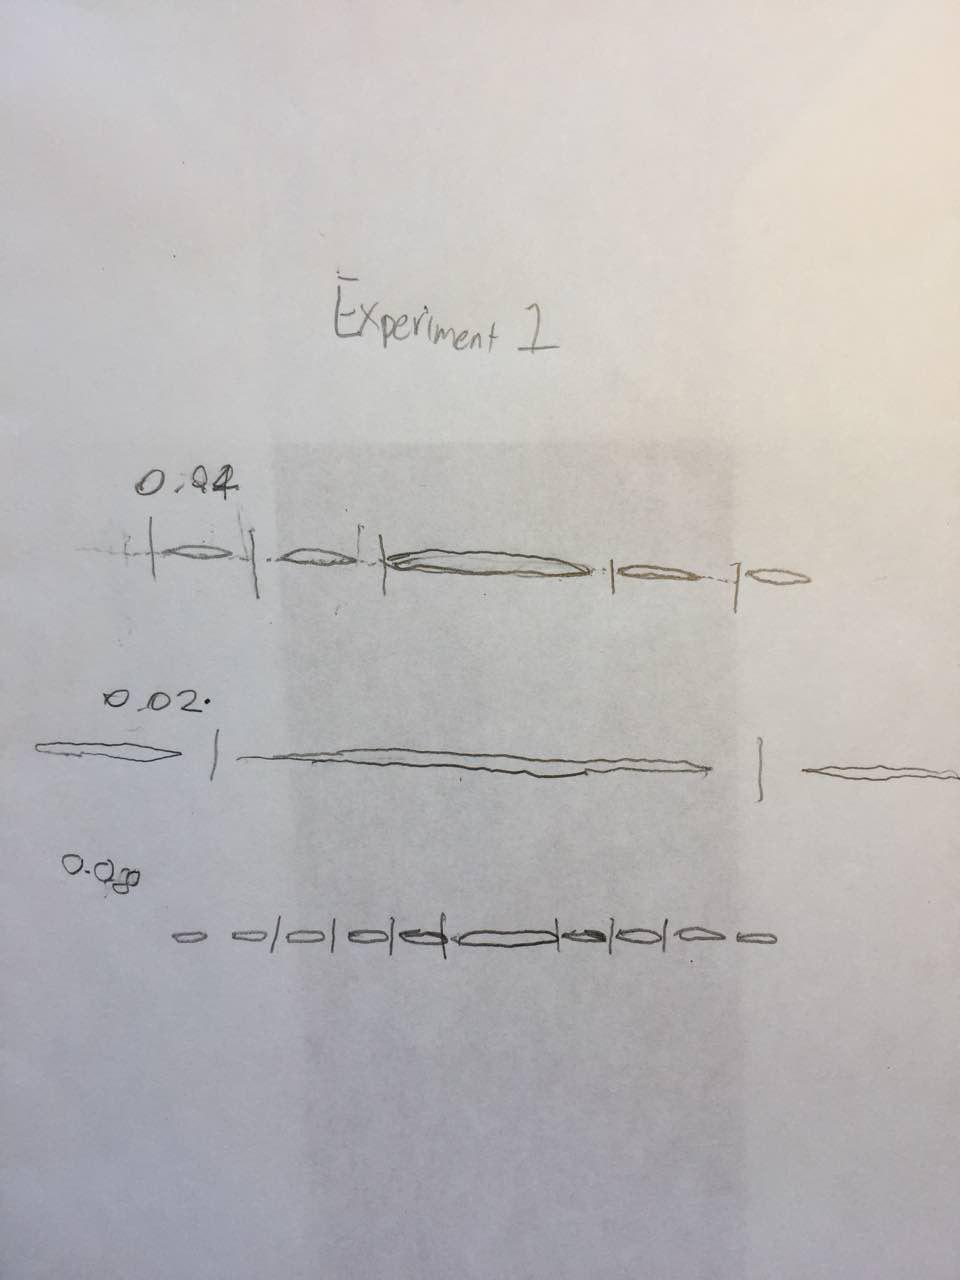
\includegraphics[scale=0.4]{exp1.jpg}
  \end{center}
  \caption{The sketches of the observed diffraction patterns. The top is of
    \SI{0.04}{\milli\meter}, the middle is of \SI{0.02}{\milli\meter}, and the
    bottom is of \SI{0.08}{\milli\meter}.}
\end{figure}

\subsubsection{Analysis}

\qq For the value of the slit-to-screen distance and the values measured for the
distance between the side orders, the error is \(\pm \SI{0.05}{\centi\meter}\)
because that is half of the smallest increment of measurement on our measuring
device, a ruler.

%-----------END EXPERIMENT 1-----------

%----------BEGIN EXPERIMENT 2----------



%-----------END EXPERIMENT 2-----------

%----------BEGIN EXPERIMENT 3----------



%-----------END EXPERIMENT 3-----------

%----------BEGIN CONCLUSION----------



%-----------END CONCLUSION-----------

\end{document}
